\subsection{Matriz DOFA}
Es una herramienta considerada sencilla la cual permite obtener una perspectiva general, de cara a la situación estratégica que debe llevar a cabo la organización. \cite{talancón} Con el fin de desarrollar los elementos de la Matriz DOFA se debe responder las siguientes preguntas de diagnóstico.

\vspace{2mm}
\begin{minipage}{0.9\textwidth}
\centering
\captionof{figure}[{Ejemplo Matriz DOFA.}]{ Ejemplo Matriz DOFA }
\label{dofa}
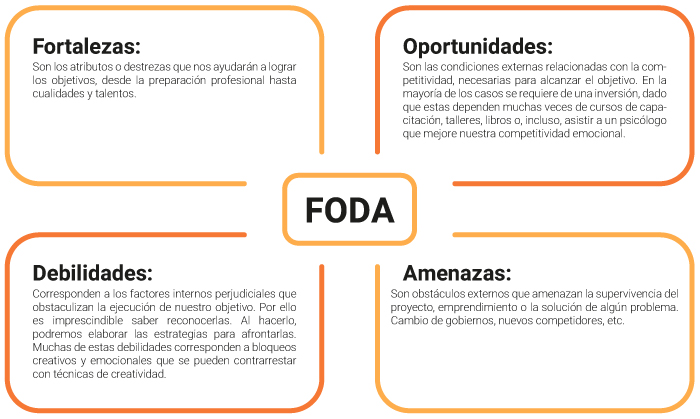
\includegraphics[width=0.7\textwidth]{Images/FODA.jpg}
\fnote{Nota. \textup{Fuente : Matriz DOFA | Qué es y cómo hacer un análisis FODA en tu empresa \cite{negoyempre_2020}}}
\end{minipage}

Las estrategias FO utilizan las fortalezas internas de la empresa para aprovechar las oportunidades externas. Las estrategias DO tienen como objetivo mejorar las debilidades internas al tomar ventaja de las oportunidades externas. La estrategia FA se basa en las fortalezas de la empresa para reducir el impacto de amenazas externas. Las estrategias DA son tácticas defensivas ya que buscan reducir las debilidades internas y evitar las amenazas externas.

\begin{minipage}{0.9\textwidth}
\centering
\captionof{table}[{ Matriz DOFA.}]{  Matriz DOFA }
\label{dofa}
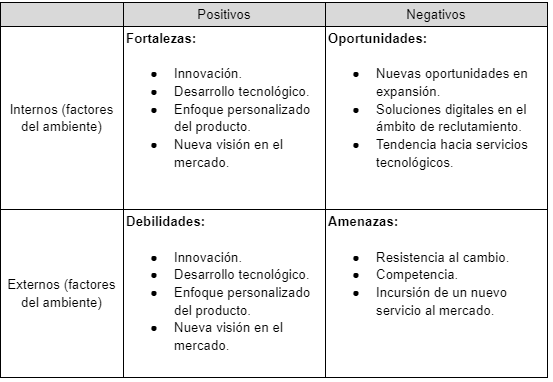
\includegraphics[width=0.7\textwidth]{Images/matrizDOFA.png}
\fnote{Nota. \textup{Fuente : Autores.}}
\end{minipage}